\documentclass[11pt,letterpaper]{article}
\usepackage[utf8]{inputenc}
\usepackage[T1]{fontenc}
\usepackage[spanish,es-nodecimaldot,es-tabla]{babel}
\usepackage{lmodern}
\usepackage[margin=2cm,top=1.8cm,bottom=1.8cm]{geometry}
\usepackage{amsmath,graphicx,booktabs,tabularx,array,enumitem,caption,hyperref}
\hypersetup{hidelinks}
\graphicspath{{figuras/}}
\captionsetup{font=small,labelfont=bf,hypcap=false}
\setlist{nosep,leftmargin=*}
\setlength{\parindent}{0pt}
\setlength{\parskip}{5pt}
\newcommand{\cod}[1]{\texttt{#1}}
\newcolumntype{L}{>{\raggedright\arraybackslash}X}
\makeatletter
\newcommand{\tableinput}[1]{\@@input #1 }
\makeatother
\newcommand{\Intercepto}{0{,}0188}
\newcommand{\Pendiente}{0{,}9966}
\newcommand{\PredAlta}{14{,}9675}
\newcommand{\MedianaTrain}{7{,}4964}
\newcommand{\MAEModelo}{0{,}0456}
\newcommand{\RMSEModelo}{0{,}0464}
\newcommand{\RdosModelo}{-29{,}0830}
\newcommand{\MAEMediana}{7{,}5167}
\newcommand{\RMSEMediana}{7{,}5167}
\newcommand{\RdosMediana}{-790109{,}6810}
\newcommand{\MAEObjetivo}{0{,}0132}
\newcommand{\RMSEObjetivo}{0{,}0156}
\newcommand{\RdosObjetivo}{-2{,}4182}

\begin{document}
\spanishplainpercent
\begin{center}
{\Large\bfseries Taller 5: tasa de transferencia en función\\del nivel de tasa configurada}\par
{\normalsize Análisis de tres pruebas TCP con iperf3}\par
Natalia Orjuela \quad | \quad Jimmy Millán \quad | \quad Santiago León
\end{center}

\section{Objetivo, alcance y protocolo}
\textbf{Objetivo.} Analizar la relación entre la tasa configurada y la tasa de transferencia medida en tres pruebas TCP, ajustar una regresión lineal y examinar fluctuaciones del caudal mediante retransmisiones y ventana de congestión (Cwnd).

\textbf{Adaptación de la actividad.} De acuerdo con la orientación del docente comunicada por la estudiante, se admite estudiar la velocidad de transferencia en función del ancho de banda. En esta entrega, esa alternativa se operacionaliza como \emph{tasa medida en función de tasa configurada}: no se conoce la capacidad nominal ni efectiva del enlace. Por tanto, los niveles de 5, 10 y 15 Mbps no representan porcentajes de utilización de la red. No se estima RTT, porque no fue medido.

\textbf{Evidencia disponible.} Se analizaron \cod{traza5.txt}, \cod{traza10.txt} y \cod{traza15.txt}, salidas de iperf3 con 300 intervalos cada una. Muestran una conexión desde A (\cod{10.124.30.129}) hacia B (\cod{10.124.30.91}), puerto 5201; los puertos de origen son 57406, 57418 y 57435. Los campos Retr y Cwnd son coherentes con pruebas TCP. La asociación de cada archivo con el nivel configurado se conserva del informe original; las trazas no contienen el comando ejecutado.

\textbf{Configuración declarada.} El informe original describe \cod{iperf3 -c 10.124.30.91 -b <N>M -t 300}, con $N\in\{5,10,15\}$, y un servidor \cod{iperf3 -s}. El comando se documenta como configuración declarada, no como registro verificado. La opción \cod{-b} establece una tasa objetivo y no mide la capacidad del enlace. No se acreditan medio, interfaz, topología física, orden cronológico, hora absoluta, número de usuarios ni versiones de las herramientas de captura.

\section{Construcción y calidad de los datos}
Cada fila de \cod{ventanas.csv} agrupa 60 intervalos consecutivos de una sesión: cinco ventanas por archivo y 15 en total. Las duraciones efectivas son 59,99--60,01 s. Las cinco ventanas de cada prueba son subdivisiones temporales, \textbf{no réplicas independientes}. Existe una sola sesión por nivel.

{\small
\begin{tabularx}{\textwidth}{p{4.5cm} L}
\toprule Campo & Definición y fuente\\ \midrule
\cod{sesion}, \cod{escenario\_mbps}, \cod{ventana} & Archivo de origen, tasa objetivo declarada y grupo de intervalos.\\
\cod{inicio\_rel\_s}, \cod{fin\_rel\_s}, \cod{duracion\_s} & Marcas relativas de iperf3; duración entre extremos.\\
\cod{bytes\_iperf\_tx\_aprox} & Suma de transferencias de texto; estimación por redondeo.\\
\cod{tasa\_medida\_mbps} & $8\,B_{\mathrm{aprox}}/(\Delta t\,10^6)$, en Mbps.\\
\cod{retransmisiones}, \cod{cwnd\_min\_kib} & Suma de Retr y mínimo de Cwnd en la ventana.\\
Campos no medidos & Hora ISO, RTT, pérdida, RX y TX de interfaz, descartes y errores: vacíos, no cero.\\
\bottomrule
\end{tabularx}}

\newpage
\section{Análisis exploratorio}
\textbf{Controles de calidad.} El programa verifica 300 intervalos continuos por archivo, duraciones positivas y cinco ventanas completas. Las retransmisiones suman exactamente 80, 200 y 123, coincidiendo con los resúmenes finales. La transferencia reconstruida suma 178,875; 357,090 y 536,930 MiB, frente a 179, 358 y 536 MBytes mostrados en los resúmenes. Las diferencias son compatibles con el redondeo acumulado de la salida de texto y no permiten recuperar bytes exactos.

Los valores KBytes y MBytes se convierten con $2^{10}$ y $2^{20}$ bytes, respectivamente; las tasas Mbps utilizan $10^6$ bits/s. Cwnd se expresa en KiB. Los bytes corresponden a la transferencia reportada por iperf3 y no a contadores del enlace ni a tráfico total del switch.

\begin{center}\small
\begin{tabular}{cccccc}
\toprule Objetivo & Tasa mediana & Rango por ventana & Retr. & Cwnd mín. & Caídas\\
(Mbps) & (Mbps) & (Mbps) & total & (KiB) & intervalos\\ \midrule
\tableinput{tabla_resumen.tex}
\bottomrule
\end{tabular}
\captionof{table}{Resumen de cinco ventanas por sesión. Caídas: tasa reportada inferior al 70\% del objetivo; criterio exploratorio, no diagnóstico de congestión.}
\end{center}

\begin{center}
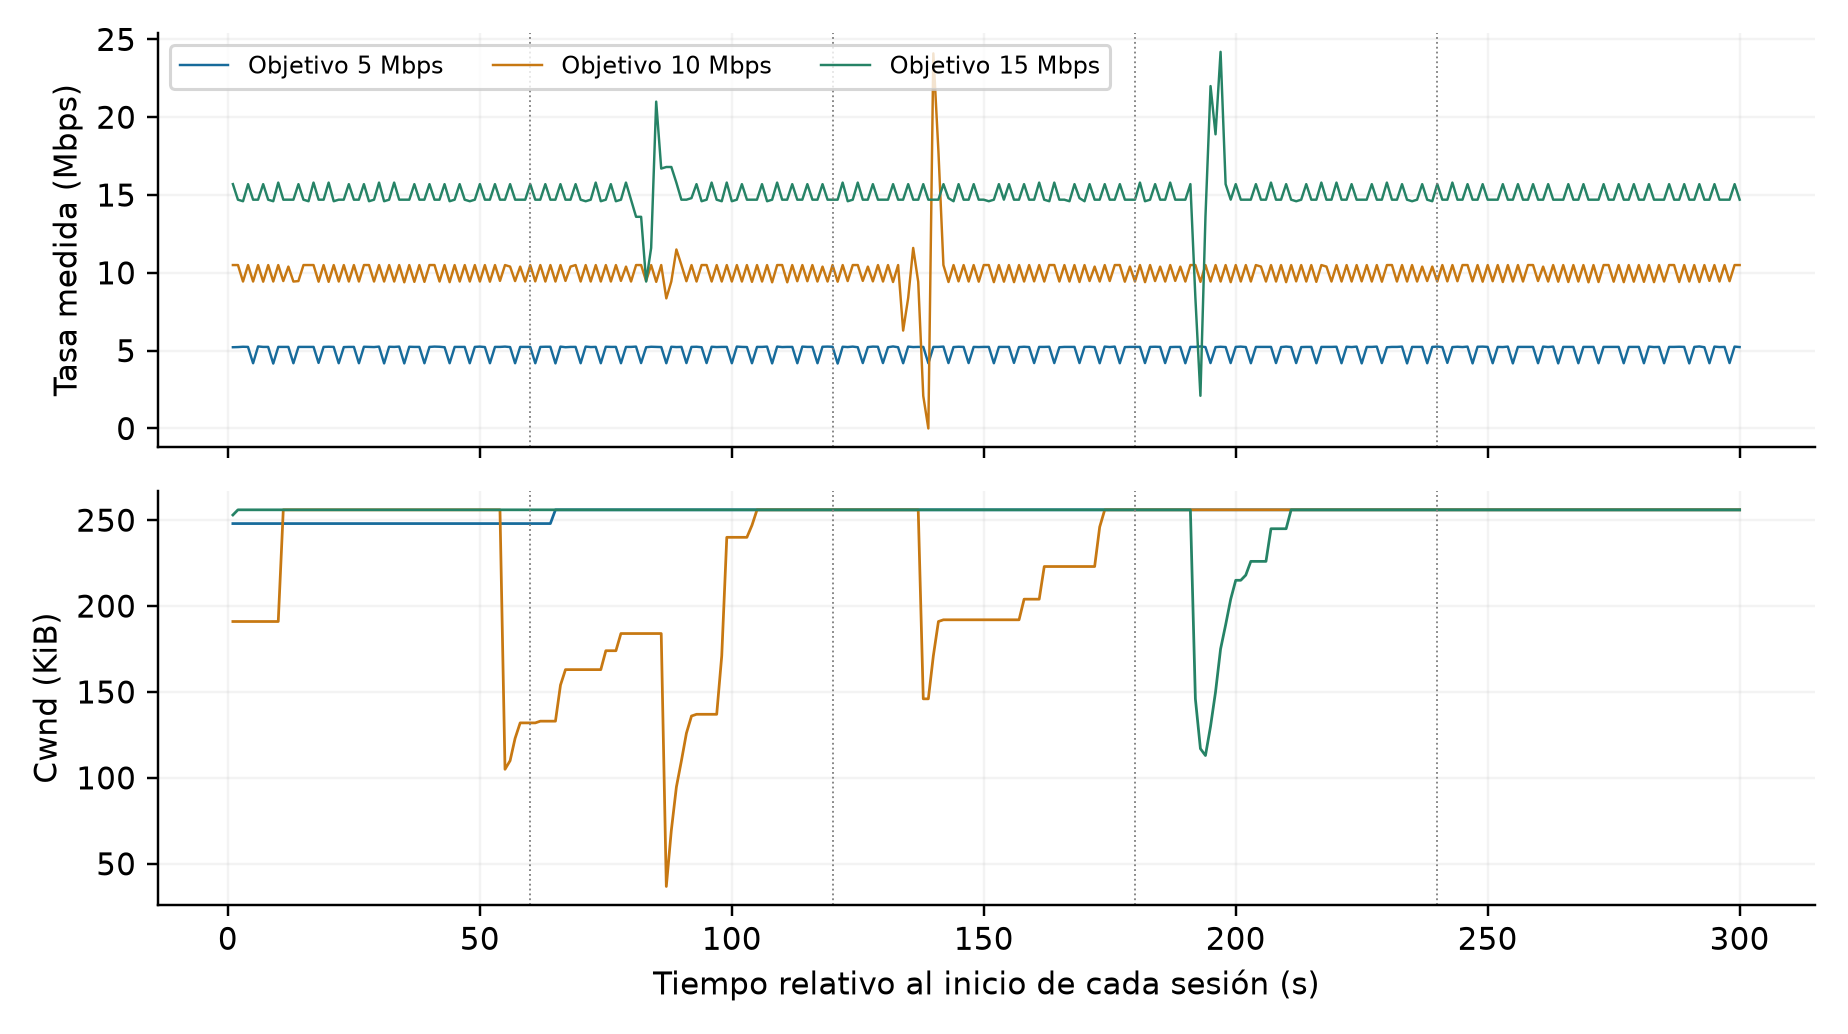
\includegraphics[width=.92\textwidth]{fig1_series.png}
\captionof{figure}{Tasa por intervalo y Cwnd. Cada curva utiliza su propio inicio de sesión; no implica simultaneidad. Líneas verticales: límites nominales de 60 s.}
\end{center}

\textbf{Interpretación.} El caudal medio sigue aproximadamente los niveles configurados. Las pequeñas oscilaciones regulares reflejan la resolución temporal y el reporte de transferencia, y no prueban congestión. Hay eventos puntuales: a 10 Mbps aparecen 2,09 Mbps entre 137,00 y 138,00 s, con 27 retransmisiones, seguidos por un intervalo sin transferencia; a 15 Mbps se observan 8,4 Mbps entre 191,01 y 192,00 s y 2,1 Mbps entre 192,00 y 193,00 s, con reducción de Cwnd. Después, el caudal se recupera. Estos eventos justifican estudiar variabilidad y TCP, pero no permiten atribuir una causa.

\newpage
\section{Relación entre tasa configurada y tasa medida}
\begin{center}
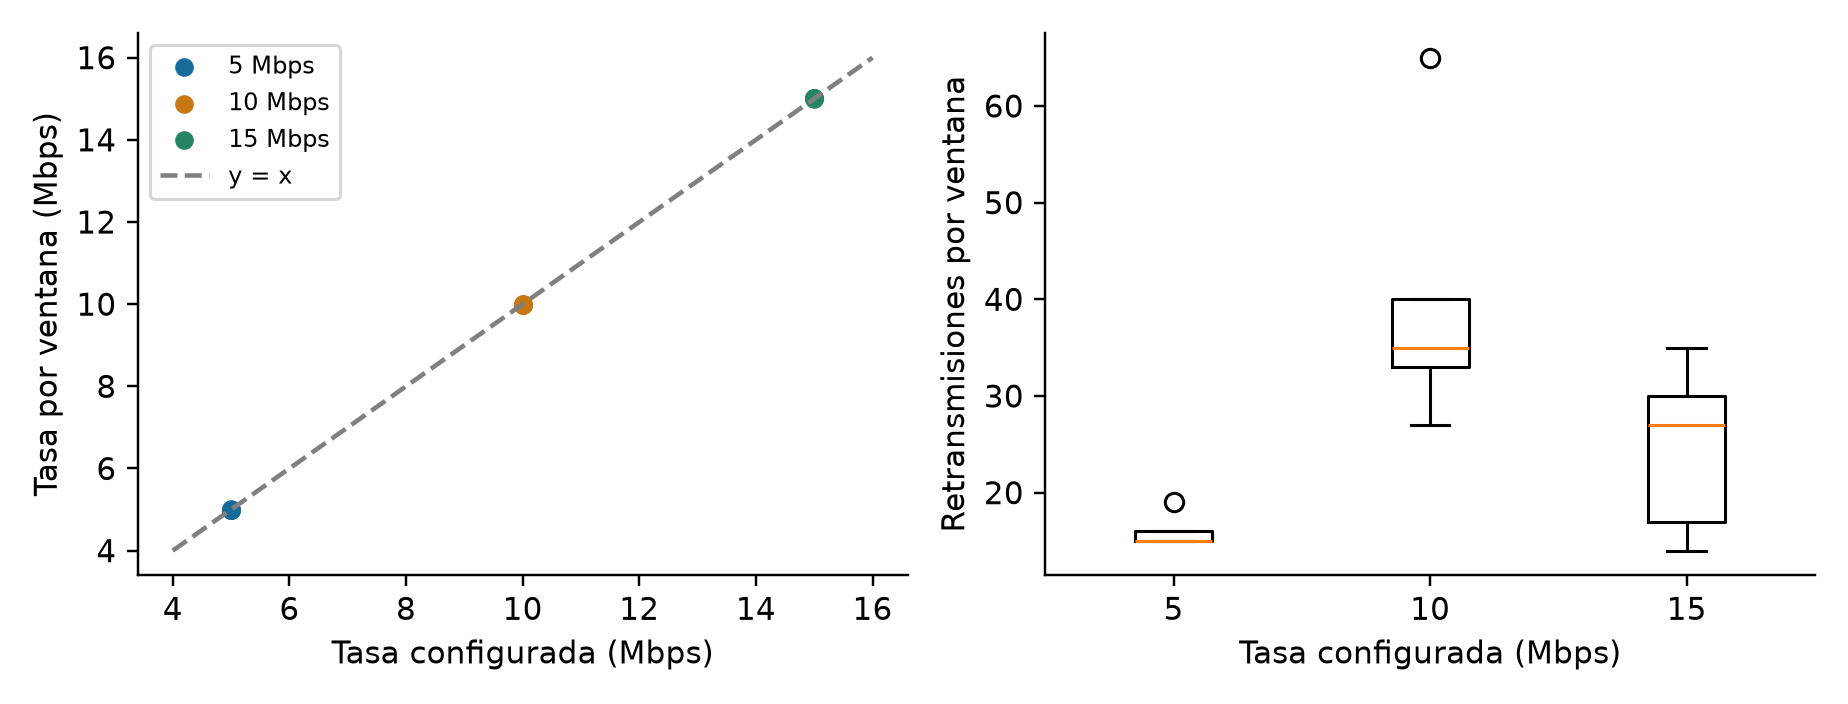
\includegraphics[width=.91\textwidth]{fig2_exploracion.png}
\captionof{figure}{Izquierda: relación objetivo--caudal, con referencia $y=x$. Derecha: distribución de retransmisiones. Ambos paneles utilizan ventanas de aproximadamente 60 s. Los puntos de tasas cercanas se superponen.}
\end{center}

La tasa mediana aumenta aproximadamente de 5,00 a 9,98 y 15,01 Mbps. En cambio, las retransmisiones no siguen un patrón monotónico: la sesión de 10 Mbps acumula más que la de 15 Mbps. Una sola sesión por nivel no permite separar el efecto de la tasa configurada del efecto de las condiciones particulares de cada sesión. Tampoco se dispone de RTT para analizar colas o latencia.

\section{Modelo y diseño de la evaluación}
\textbf{Variables.} Se utiliza $x=$ tasa configurada (Mbps) y $y=$ tasa medida por ventana (Mbps). Las retransmisiones se mantienen como evidencia complementaria, no como sustituto de RTT. Se ajusta por mínimos cuadrados:
\[
\widehat y=\beta_0+\beta_1x = \Intercepto + \Pendiente\,x.
\]
La pendiente es adimensional; el intercepto se expresa en Mbps. Su interpretación se restringe a los niveles estudiados: no se midió un escenario de 0 Mbps ni se debe atribuir significado físico al intercepto fuera de ese contexto.

\textbf{Separación por sesiones completas.} Las sesiones de 5 y 10 Mbps se usan para entrenamiento (10 ventanas); la sesión completa de 15 Mbps se reserva para evaluación (5 ventanas). No hay sesiones compartidas entre conjuntos. Esta decisión evita mezclar segmentos de una misma prueba, pero mantiene dos limitaciones: solo hay dos valores de $x$ en entrenamiento y las cinco observaciones de evaluación pertenecen a una única sesión.

El rango de entrenamiento es $x\in[5,10]$ Mbps y la evaluación ocurre en $x=15$ Mbps: es \textbf{extrapolación retrospectiva}. Las trazas ya existían cuando se preparó el análisis; no hubo predicción registrada antes de medir. La ausencia de marcas de reloj impide afirmar una evaluación cronológica hacia el futuro. La partición queda explícita en el código, sin ajuste posterior usando la sesión reservada.

\textbf{Referencias.} Se compara con (a) la mediana del caudal de entrenamiento ($\MedianaTrain$ Mbps), como referencia constante, y (b) $\widehat y=x$, como referencia operativa de seguimiento del objetivo. La segunda utiliza el nivel configurado conocido y no resultados de la sesión reservada. Si el caudal sigue directamente ese nivel, una regresión puede ser innecesaria.

\newpage
\section{Evaluación retrospectiva a 15 Mbps}
Para $x=15$ Mbps, el modelo produce $\widehat y=\PredAlta$ Mbps en las cinco ventanas. La entrada es el nivel configurado declarado, no una tasa futura medida. La tabla muestra las observaciones reservadas y el residuo $e=y-\widehat y$.

\begin{center}\small
\begin{tabular}{ccccc}
\toprule Ventana & Medido & Predicho & Residuo & Error absoluto\\
 & (Mbps) & (Mbps) & (Mbps) & (Mbps)\\ \midrule
\tableinput{tabla_predicciones.tex}
\bottomrule
\end{tabular}
\captionof{table}{Resultados por ventana en la única sesión reservada.}
\end{center}

\begin{center}\small
\begin{tabular}{lrrr}
\toprule Método & MAE (Mbps) & RMSE (Mbps) & $R^2$\\ \midrule
Regresión lineal & \MAEModelo & \RMSEModelo & \RdosModelo\\
Mediana de entrenamiento & \MAEMediana & \RMSEMediana & \RdosMediana\\
Objetivo ($\widehat y=x$) & \MAEObjetivo & \RMSEObjetivo & \RdosObjetivo\\
\bottomrule
\end{tabular}
\captionof{table}{Métricas calculadas exclusivamente sobre cinco ventanas de la sesión de 15 Mbps.}
\end{center}

\begin{center}
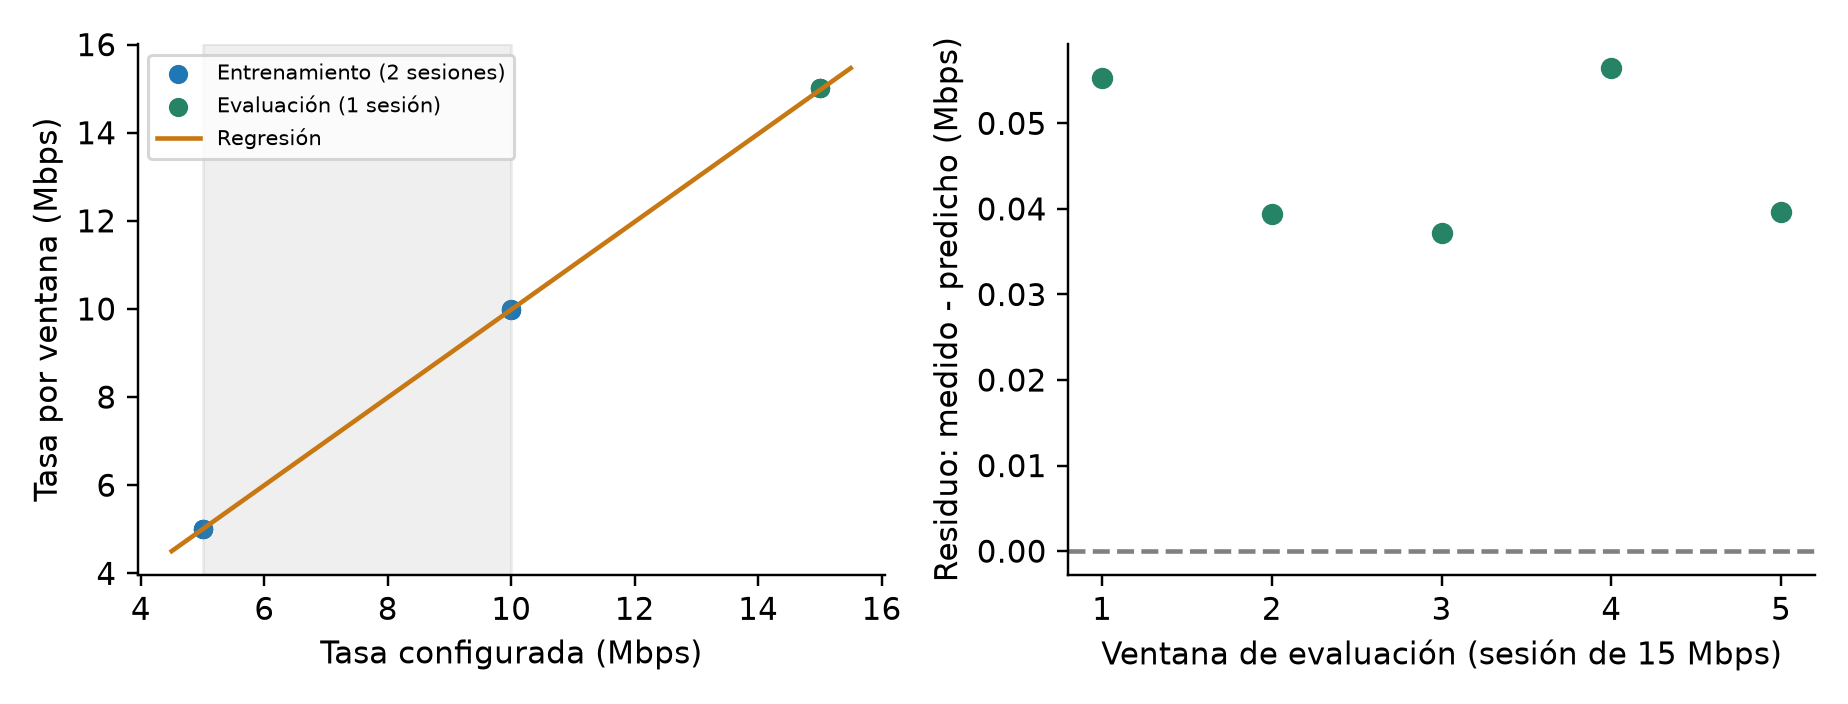
\includegraphics[width=.91\textwidth]{fig3_modelo.png}
\captionof{figure}{Ajuste y extrapolación (izquierda); residuos por ventana reservada (derecha). Franja gris: rango de entrenamiento.}
\end{center}

\textbf{Lectura.} La regresión presenta errores absolutos pequeños respecto de 15 Mbps y supera a la referencia constante, pero la referencia $\widehat y=x$ tiene menor error. El ajuste no demuestra una ventaja práctica frente a usar directamente la tasa objetivo. El $R^2$ negativo se explica porque el modelo no reproduce las pequeñas diferencias entre ventanas de una sesión casi constante: su suma de errores cuadrados supera la de predecir la media de la prueba. Un error absoluto pequeño y un $R^2$ negativo pueden coexistir; ninguno acredita generalización a otras sesiones.

\textbf{¿Fue una prueba congestionada?} 15 Mbps es el nivel más alto observado, no una condición de congestión confirmada. El caudal agregado sigue el objetivo y se recupera de las caídas. Sin capacidad conocida, RTT, descartes, carga total ni repeticiones no se puede confirmar saturación sostenida ni identificar su causa. Tampoco se identifica un umbral para justificar un modelo segmentado con estos datos.

\newpage
\section{Conclusiones, límites y reflexión}
\begin{enumerate}
\item En las tres sesiones disponibles, la tasa media de transferencia aumenta aproximadamente en proporción al nivel configurado de 5, 10 y 15 Mbps. Esto describe el comportamiento de la conexión analizada, no la capacidad disponible ni la utilización del enlace completo.
\item La regresión entrenada con dos niveles aproxima el caudal de la sesión de 15 Mbps, pero no mejora la referencia de seguimiento del objetivo. El resultado favorece un análisis descriptivo y no justifica afirmar una capacidad predictiva robusta.
\item Las caídas de caudal, las retransmisiones y las reducciones de Cwnd muestran perturbaciones transitorias. No hay evidencia suficiente para atribuirlas a otros usuarios, interferencia o congestión causada por la prueba.
\item La evaluación usa sesiones separadas, pero es retrospectiva, extrapola y solo contiene una sesión reservada. Las ventanas no aumentan el número de réplicas independientes. El redondeo de las trazas limita la precisión de las tasas reconstruidas.
\end{enumerate}

\textbf{Mejora del protocolo.} Registrar medio, interfaz, capacidad de referencia, topología, marcas ISO y versiones; realizar al menos tres sesiones independientes por nivel y alternar el orden; conservar salidas JSON para evitar redondeo; medir contadores y, si se desea estudiar calidad, RTT y pérdida en paralelo. Reservar sesiones completas, registrar la predicción antes de medir y evaluar distintos niveles autorizados. Estimar congestión requeriría evidencia adicional y un entorno controlado.

\textbf{Mediciones reales y datos ausentes.} Las tres trazas contienen 900 intervalos con transferencia, tasa, retransmisiones y Cwnd. No se dispone de mediciones de RTT, pérdida ICMP, contadores de interfaz, captura PCAP, línea base sin carga, capacidad del enlace ni marcas absolutas. Estos datos no se reconstruyen ni se sustituyen por valores inventados.

\textbf{Preguntas de reflexión.}
\begin{enumerate}
\item \emph{¿Por qué los bytes de A no determinan la utilización del switch?} La conexión observada no recoge todo el tráfico de sus puertos. La utilización requiere conocer capacidad, dirección y tráfico relevante; iperf3 reporta transferencia de su prueba, no todos los bytes de interfaz.
\item \emph{¿En qué difieren RTT, latencia unidireccional y respuesta de aplicación?} RTT mide ida y vuelta de una sonda; la latencia unidireccional mide un trayecto y requiere sincronización para medición directa; la respuesta de aplicación incorpora intercambios de red y procesamiento. Ninguna de estas métricas se deduce del caudal medido.
\item \emph{¿Por qué un MAE pequeño no garantiza acierto bajo congestión?} La evaluación puede cubrir solo condiciones estables. Un régimen con colas o pérdidas puede cambiar la relación y requerir otras variables. Las presentes pruebas no verifican ese cambio de régimen.
\item \emph{¿Qué cambiaría con Wi-Fi?} Se registrarían banda, canal, señal, tasa de enlace y posición, con más sesiones y control del tráfico concurrente. La competencia por el medio y las condiciones radioeléctricas dificultan atribuir las variaciones de caudal a una sola causa.
\end{enumerate}

\end{document}
